\section{\acl{rtsp}}
\acs{rtsp} ist ein Netzwerkprotokoll zum Aufbauen und Verwalten von Netzwerkverbindungen zur Übertragung kontinuierlicher Medien-Daten (Streams).
Dieses Netzwerkprotokoll ist im \acs{ietf}-Dokument \citetitle{ietf-rtsp} festgelegt. 
Es wurde gemeinsam von \citeauthor{ietf-rtsp} entwickelt. \cite[vgl.][]{ietf-rtsp}\par

\subsection{\acs{rtsp} Version 2}
Im Zuge dieser Diplomarbeit wird die erste Version des \acs{rtsp}-Protokolls verwendet.
Neben der verwendeten Version 1 existiert auch eine neue Version 2, welche im \acs{ietf}-Dokument \citetitle{ietf-rtsp-2} definiert ist. Die neue Version wurde von \citeauthor{ietf-rtsp-2} erarbeitet. \cite[vgl.][]{ietf-rtsp-2}\par
Es wurde dennoch die erste Version verwendet, da die Stationen dieses bereits verwenden und die neue Version nicht rückwärtskompatibel ist.\par

\acs{rtsp} wird in der Industrie vielseitig verwendet, um Live-Übertragungen von Überwachungskameras zu verwalten. Eine weitere Anwendung des \acs{rtsp} Protokolls ist das Streamen von Medien-Daten zu einem Server, der diese dann beispielsweise transcodiert oder aufnimmt.

\subsection{Anfragen-Aufbau}
Das \acs{rtsp}-Protokoll definiert mehrere Anfragen zur Verwaltung der Netzwerkverbindung.
Diese Anfragen werden, ähnlich wie beim \acs{http}, in unverschlüsseltem Plain-Text verschickt.
In Tabelle \ref{tab:rtsp-req} sind sämtliche Anfragen des \acs{rtsp}-Protokolls und deren Übertragungsrichtung aufgelistet.
Die in Tabelle \ref{tab:rtsp-req} verwendeten Kurzbezeichnungen haben folgende Bedeutung:
\paragraph{Richtung:} C\dots Client, S\dots Server
\paragraph{Objekt:}P\dots Präsentation, S\dots Stream
\begin{table}[H]
    \centering\begin{tabular}{|r|c|c|l|}
        \hline%-----------------------------------------------------------
        Methode         &Richtung                           &Objekt &Verbindlichkeit\\
        \hline%-----------------------------------------------------------
        DESCRIBE        &C$\rightarrow$S                    &P,S    &empfohlen\\
        ANNOUNCE        &C$\rightarrow$S, S$\rightarrow$C   &P,S    &optional\\
        GET\_PARAMETER  &C$\rightarrow$S, S$\rightarrow$C   &P,S    &optional\\
        OPTIONS         &C$\rightarrow$S, S$\rightarrow$C   &P,S    &erfordert, (S$\rightarrow$C: optional)\\
        PAUSE           &C$\rightarrow$S                    &P,S    &empfohlen\\
        PLAY            &C$\rightarrow$S                    &P,S    &erfordert\\
        RECORD          &C$\rightarrow$S                    &P,S    &optional\\
        REDIRECT        &S$\rightarrow$C                    &P,S    &optional\\
        SETUP           &C$\rightarrow$S                    &S      &erfordert\\
        SET\_PARAMETER  &C$\rightarrow$S, S$\rightarrow$C   &P,S    &optional\\
        TEARDOWN        &C$\rightarrow$S                    &P,S    &erfordert\\
        \hline%-----------------------------------------------------------
    \end{tabular}
    \caption{Anfrage-Arten des \acs{rtsp}-Protokolls}
    \label{tab:rtsp-req}
\end{table}
Das Aussehen einer solchen Anfrage wird anhand des Beispiels der DESCRIBE-Methode veranschaulicht.
Der Client beginnt die Anfrage mit dem \acs{url} des Medien-Streams, den er abrufen möchte und teilt dem Server mit, welche Formate er versteht.
\begin{minted}{text}
C->S: DESCRIBE rtsp://server.example.com/fizzle/foo RTSP/1.0
    CSeq: 312
    Accept: application/sdp, application/rtsl, application/mheg
\end{minted}
Der Server antwortet auf diese Anfrage mit dem Session Descriptor, der alle wichtigen Informationen des Medien-Streams beinhaltet, wie zum Beispiel Video- und Audio-Format, Übertragungsmethode, sowie allgemeine Informationen wie Titel und Beschreibung.
\begin{minted}{text}
S->C: RTSP/1.0 200 OK
    CSeq: 312
    Date: 23 Jan 1997 15:35:06 GMT
    Content-Type: application/sdp
    Content-Length: 376

    v=0
    o=mhandley 2890844526 2890842807 IN IP4 126.16.64.4
    s=SDP Seminar
    i=A Seminar on the session description protocol
    u=http://www.cs.ucl.ac.uk/staff/M.Handley/sdp.03.ps
    e=mjh@isi.edu (Mark Handley)
    c=IN IP4 224.2.17.12/127
    t=2873397496 2873404696
    a=recvonly
    m=audio 3456 RTP/AVP 0
    m=video 2232 RTP/AVP 31
    m=whiteboard 32416 UDP WB
    a=orient:portrait
\end{minted}

\section{LibVLC Sharp}
LibVLC ist ein Multimedia-Rahmenwerk der Non-Profit-Organisation VideoLAN, welche durch den VLC Media Player und dessen Funktionsumfang bekannt wurde. Der VLC Media Player funktioniert sozusagen als grafische Oberfläche zur LibVLC-Programmbibliothek.
Die Bibliothek beinhält viele nützliche Funktionen, darunter die folgenden:
\begin{itemize}
    \item Videos nahezu beliebigen Formates decodieren und darstellen
    \item Video und Audio aufnehmen und transcodieren für die weitere Verwendung
    \item Live-Streaming von Video-Daten, Webcam-Bild und Mikrofon-Ton.
\end{itemize}    
LibVLC ist eine Bibliothek für die C-Sprache. Um diese in einem C\#-Projekt verwenden zu können sind Bindings notwendig, welche Zugriff auf die C-Bibliothek geben.
LibVLC wurde von der Non-Profit-Organisation VideoLAN entwickelt und erstmals am 1. Februar 2001 veröffentlicht.\cite[vgl.][]{libvlc-release}\par

Im Xamarin.Forms-Projekt wird die zum Zeitpunkt der App-Entwicklung aktuelle Version 3.4.2 der LibVLC Sharp Bindings verwendet. Bindings erlauben es dem Programmierer, auf Programmbibliotheken zuzugreifen, welche für eine andere Sprache geschrieben wurden. Man kann sich Bindings wie Kleber vorstellen, der die Funktionen der einen Programmiersprache mit denen der anderen Sprache verbindet. Die Version 3.4.2 ist inzwischen nicht mehr die neueste Version, jedoch ist sie in Hinsicht auf Funktionalität deckungsgleich mit der neuesten Version.\par

\subsection{Erwähnenswerte Funktionen}
Die LibVLC-Sharp-Bindings ermöglichen die Verwendung des MVVM-Modells, welches vom WPF- und Silverlight-Architekten John Gossman im Jahr 2005 auf seinem Blog vorgestellt wurde. \cite[vlg.][The Evolution of Model-View-ViewModel]{msdoc-mvvm}
Die Philosophie hinter diesem Modell ist, die Oberfläche (View) bis auf wenige Schnittstellen komplett vom eigentlichen Code zu trennen.
Dies ermöglicht es ohne größeren Aufwand, die Oberfläche zu ändern oder gar auszutauschen.
Folgende Terminologie wird in diesem Zusammenhang verwendet:
\begin{itemize}
\item Models … beinhalten die Programmdaten. Meist werden einfache Klassen oder Strukturen hierfür verwendet.
\item Views … Die grafische Oberfläche und deren Elemente wie Buttons, TextBoxen, …
\item ViewModels … wandeln die Daten der Models so um, dass sie von der Oberfläche dargestellt werden können. ViewModels sind meist als Klasse ausgeführt.
\end{itemize}

Die Daten der Oberfläche und die Daten des Models bleiben zueinander konsistent. Sobald sich ein Wert auf einer Seite ändert, wird er sofort auf der anderen aktualisiert.
\begin{figure}[H]
    \centering
    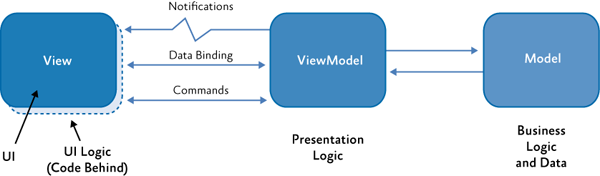
\includegraphics[width=.9\linewidth]{images/software_module/MVVM.png}
    \caption{Datenfluss MVVM}
\end{figure}
Das MVVM-Modell bietet sich auch an, wenn die Daten des Programms oft in eine andere Form gebracht werden müssen, bevor sie dargestellt werden können. Zum Beispiel wird vom Model die aktuelle Zeit als Ganzzahl abgespeichert, welche nur die vergangenen Millisekunden seit einem bestimmten Zeitpunkt zählt; um die Zeit allerdings darstellen zu können, muss diese Ganzzahl zuerst in ein lesbares Datumsformat gebracht werden. Diese Aufgabe würde das ViewModel übernehmen.

\subsection{Nachteile}
Sowohl die ursprüngliche LibVLC-Bibliothek, als auch die entsprechenden C\#-Bindings sind auf der offiziellen Dokumentationsseite nur spärlich dokumentiert.\cite[vgl.][]{libvlc-sharp-doc}
%quelle
Beispielsweise verwenden alle Beispielprojekte der LibVLC Sharp Bindings das MVVM-Modell, daher ist nicht bekannt, ob eine Implementierung ohne dieses Modell überhaupt möglich ist.
Weiters sind die einzelnen Funktionen zwar auf der Dokumentationsseite aufgelistet, allerdings nicht sehr ausführlich beschrieben. \cite[vgl.][]{libvlc-sharp-doc}

\subsection{Alternativen}
Während der Recherche wurden wenige Alternativen gefunden. Diese Alternativen sind jedoch seit langem nicht mehr in Entwicklung und sind daher nicht für die Verwendung empfohlen. Die LibVLC-Bibliothek ist momentan die einzige kostenfreie Variante, \acs{rtsp}-Streams mit Xamarin auf dem Mobilgerät abspielen zu können. Es gibt Bibliotheken von VASTreaming, jedoch sind diese kostenpflichtig zu erwerben, was für diese Diplomarbeit keine Option ist. \cite[vgl.][Pricing]{vastreaming}

\section{GStreamer}
\subsection{Modularität}
GStreamer ist ein extrem leistungsfähiges und vielseitiges Framework zur Erstellung von Medien-Streaming-Anwendungen.
Viele der Vorzüge des GStreamer-Frameworks liegen in seiner Modularität:
GStreamer kann neue Plugin-Module nahtlos integrieren.
Aber da Modularität und Leistungsfähigkeit oft mit einem Preis für eine größere Komplexität einhergehen, ist das Schreiben neuer Anwendungen nicht immer einfach.
\cite[aus dem Englischen übersetzt]{gstreamer}\par

GStreamer ist Pipeline-basiert, d.h. die Funktion wird mit einer Vielzahl von hintereinander geschalteten Filtern bestimmt.
Eine Pipeline hat immer einen Eingang (Source) und einen oder mehrere Ausgänge.
Zwischen diesen können sich beliebig viele Filter befinden, die unterschiedlichste Funktionen haben können:
\begin{itemize}
    \item Signale de- und encodieren (Codec, z.B. x264enc)
    \item Größe und Position von Videos verändern (Caps, z.B. video/x-raw)
    \item die Pipeline in zwei Teile auftrennen, z.B. in Video und Audio (Demux)
    \item Daten zu einem Netzwerk-Paket zusammenbündeln (z.B. rtph264pay)
    \item etc.
\end{itemize}
Ein Filter hat bestimmte Ein- und Ausgangsformate, die er unterstützt.
Als Beispiel nehmen wir den H264-Encoder:
dieser unterstützt für das Eingangssignal RAW-Video, also decodierte Binärdaten. Am Ausgang kommt logischerweise ein H264-codierter Video-Stream heraus.\par

\subsection{Version}
Das GStreamer-Rahmenwerk wird aktuell vom GStreamer-Team fortlaufend upgedatet und verbessert.
Die erste Version des GStreamer-Rahmenwerks wurde im Jahr 2001 mit der Versionsnummer 0.1.0 veröffentlicht.
Im Jahr 2012 kam eine große Umstellung, bei der grundlegende Teile des Rahmenwerks ausgetauscht wurden, wodurch einige Teile nicht mehr kompatibel waren.
Ab diesem Zeitpunkt begann die Versionsnummer mit 1.x.x, um die neuen Versionen deutlich von den Vorgängern abzutrennen.
Die aktuelle Version des GStreamer-Rahmenwerks zum Verfassungszeitpunkt dieser Arbeit ist die Version 1.16.2.\par

Aktuell wird die Version 1.16.2 verwendet. Da aber alle 1.x.x-Versionen mehr oder weniger miteinander kompatibel sind, kann sich das ändern, sobald ein neues Update veröffentlicht wird. Es gibt keinen besonderen Grund auf genau dieser Version zu bleiben.\par

\subsection{Alternativen}
Es wurden während der Recherche einige mögliche Alternativen für das GStreamer-Rahenwerk gefunden:
\begin{itemize}
    \item FFmpeg, ein Multimedia-Rahmenwerk, das vor allem im Bereich Transcodierung Verwendung findet. Es bietet alle Funktionen des GStreamer-Rahmenwerks an.
    \item LibVLC, die Grundlage des VLC Media Players, welche vor allem zur Wiedergabe verwendet wird. Diese Bibliothek kann zur Transcodierung und Live-Übertragung genutzt werden, ist allerdings nicht dafür optimiert.
\end{itemize}

\subsection{Vorteile}
GStreamer wird in diesem Projekt verwendet, da bei Live-Video-Übertragung möglichst wenig Latenz vorkommen soll.
Das GStreamer-Rahmenwerk ist in dieser Hinsicht den anderen Multimedia-Rahmenwerken weit voraus.
Zusätzlich gibt es von GStreamer keine einschränkenden Vorgaben, was Ein- und Ausgangsformat betrifft.
Es kann jede beliebige Quelle mit jedem beliebigen Output verknüpft werden, solange die richtige Pipeline verwendet wird.
Weiters ist das Projekt quelloffen, d.h. man ist in Bezug auf die Installationsdateien nicht auf den Hersteller angewiesen, sondern kann das Programm selbst für die jeweilige Plattform kompilieren, wenn der Hersteller das noch nicht getan hat.
Außerdem kann jeder Entwickler Vorschläge für Änderungen am Code sowie Bugfixes vorbringen.
\subsection{Funktionsweise}
Die detaillierte Funktionsweise des GStreamer-Rahmenwerks lässt sich am besten anhand eines realistischen Beispiels erklären.
In diesem Beispiel wird ein in Echtzeit generiertes Testvideosignal zuerst auf 1280x720 Pixel vergrößert und danach als H264-encodierter Stream via RTP verschickt.
Mit dem Kommandozeilen-Programm \texttt{gst-launch-1.0.exe} kann ohne großen Aufwand eine Pipeline aufgebaut werden:
\begin{minted}{csharp}
    gst-launch-1.0 videotestsrc ! video/x-raw,width=1260,height=720,framerate=20/1 ! autovideoconvert ! queue ! x264enc tune=zerolatency bitrate=4096 speed-preset=superfast ! queue ! rtph264pay config-interval=1 mtu=1300 ! udpsink host=127.0.0.1 port=5000
\end{minted}
Der Filter \enquote{queue} wird hier verwendet, um vor und nach dem Encoding-Vorgang ein kurzes Video-Segment in einem Zwischenspeicher zu behalten. Dies ist notwendig, da der H264-Codec mehrere Video-Frames auf einmal komprimiert.

\subsection{Zusatzmodul}
gst-rtsp-server ist ein Zusatzmodul für das GStreamer- Rahmenwerk, welches die Verwendung des \acs{rtsp}-Protokolls für Server-Applikationen bereitstellt.
Mit diesem Modul können Medien-Streams, welche mit GStreamer verarbeitet wurden, mittels dem \ac{rtsp}Protokoll den Netzwerk bereitzustellen.

%TODO

\section{Live555 Proxy}
Ein \acs{rtsp}-Stream ist grundsätzlich eine Unicast-Verbindung zwischen Server und Client.
Falls mehrere Clients den gleichen Medien-Stream abrufen möchten, muss der Server diesen für jeden Client einzeln transcodieren und verschicken.
Dies stellt eine große Belastung für den Server und dessen Internetanbindung dar.
Mit Hilfe eines Proxy-Servers muss der Medien-Stream nur einmal verarbeitet werden, bevor er dann an die einzelnen Clients verteilt wird.\par

Der Live555 Proxy Server ist eine quelloffene Applikation, welche für genau diese Aufgabe von Live Networks Inc. entwickelt wurde.
Mit Hilfe des Live555 Proxy Servers wird ein \acs{rtsp}-Stream einmalig eingelesen und an alle verbundenen Clients verteilt.
Dadurch bleibt die \acs{cpu}-Belastung des Servers unabhängig von der Anzahl der verbundenen Clients, wodurch er unter Umständen mehrere verschiedene Streams bereitstellen könnte. Für jeden Medien-Stream, den der Server anbietet, wird eine weitere Live555-Proxy-Server-Instanz benötigt.\par

Das ursprüngliche Veröffentlichungsdatum des Live555 Proxy Servers konnte nicht gefunden werden.
Bei Analyse der Google-Such-Trends zum Begriff Live555 wurde festgestellt, dass Suchanfragen mit Oktober 2005 gestartet haben.
Daher lässt sich vermuten, dass das Programm kurz vor diesem Zeitpunkt veröffentlicht wurde. \cite[vgl.][Interest over time]{live555-trends}

Neben dem Live555 Proxy Server entwickelt das Unternehmen mehrere Projekte:
\begin{itemize}
    \item Live555 Media Server, mit dem lokale Medien-Dateien per \acs{rtsp} dem Netzwerk bereitgestellt werden können.
    \item liveCaster, zur Multicast-Übertragung von MP3-Dateien
    \item diverse Kommandozeilenprogramme zum Senden und Empfangen von Echtzeit-Streams
\end{itemize}
Die von Live Networks Inc. entwickelten Programme und Bibliotheken finden in vielen bekannten Applikationen Anwendung, darunter auch der VLC Media Player mit der dazugehörigen LibVLC. In diesem Programm werden die Live555-Bibliotheken zum Empfangen und Entschlüsseln von \acs{rtsp}-Streams genutzt.